\documentclass[../Main.tex]{subfiles}

\begin{document}
\author{Total Internal Reflection} %use author for title of lesson
\date{Year 1 Topic 17} %use date to refer to topic in main booklet

\section{Total Internal Reflection} %Section is the title of the lesson repeated, ready for the main contents page.

\begin{frame}{Reflection and Refraction recap}
    Recall the law of reflection \pause
    \begin{block}{Law of Reflection}
    The angle of incidence is equal to the angle of reflection. \begin{equation*}
        \theta_i = \theta_r
    \end{equation*}
    \end{block}
    And the law of refraction - `Snell's Law' \pause
    \begin{block}{Snell's Law}
    \begin{equation*}
        n sin \theta = k
    \end{equation*} \center{or}
    \begin{equation*}
        n_1 sin(\theta_1) = n_2 sin(\theta_2)
    \end{equation*}
    \end{block}
\end{frame}

\begin{frame}{Refraction}
    What happens to a light ray crossing the boundary between two mediums? \pause 
    \newline \newline
    Generally we get some refraction and partial reflection, showing our refracted ray as a solid line, and a partial reflection as a dashed line. 
    
    \begin{figure}
        \centering
        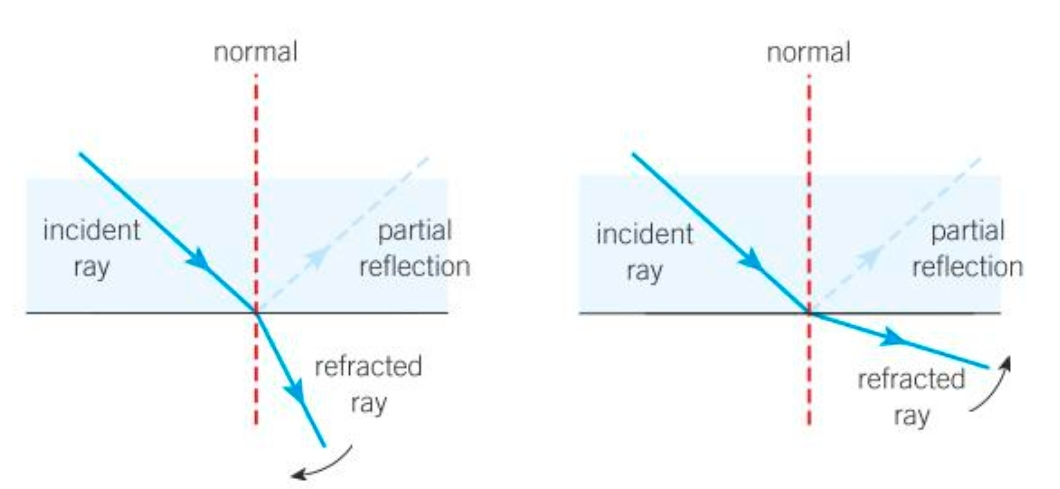
\includegraphics[height=3cm]{Waves_Images/lawofrefraction.jpg}
    \end{figure}
    
    But this is not always the case...
\end{frame}

\begin{frame}{Reflection back into a medium}
    Sometimes, if the light is at a particular angle, we might find that all of the light is reflected back inside the medium, never leaving the medium it is currently in. \pause
    \begin{block}{Demo}
    Lets see if we can get this working... 
    \end{block} \pause
    \begin{figure}
        \centering
        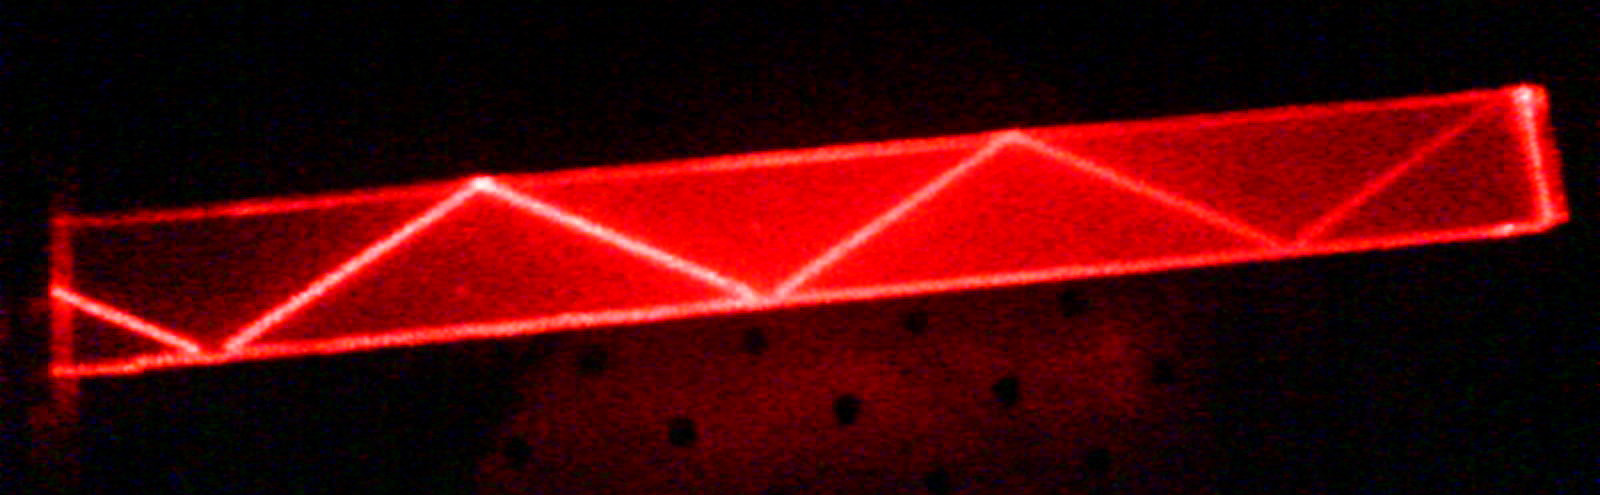
\includegraphics[width=\textwidth]{Waves_Images/totalinternalreflectiondemo.jpg}
    \end{figure}
\end{frame}

\begin{frame}{Total Internal Reflection}
    This is called total internal reflection (TIR). There are some conditions for TIR to occur - and you are expected to be able to recall and state these in exams:
    \begin{itemize}
        \item Light must be travelling from a medium with a higher optical density to a lower ($n_2<n_1$).
        \item The light ray must meet the boundary at an angle greater than or equal to the \emph{critical angle} ($\theta \geq C$).
    \end{itemize}\pause
    \begin{block}{Critical Angle}
    The critical angle is the minimum angle of incidence required for total internal reflection to occur. It is calculated as 
    \begin{equation*}
        sin (C) = \frac{n_2}{n_1}
    \end{equation*}
    *note that for most exam questions, the second medium is air, hence the formula book states $sin (C) = \frac{1}{n}$, where n is the refractive index of the medium light is leaving.
    \end{block}
\end{frame}

\begin{frame}{TIR}
Remember -- the angle of incidence is still defined as the angle between the light ray and normal line
    \begin{figure}
        \centering
        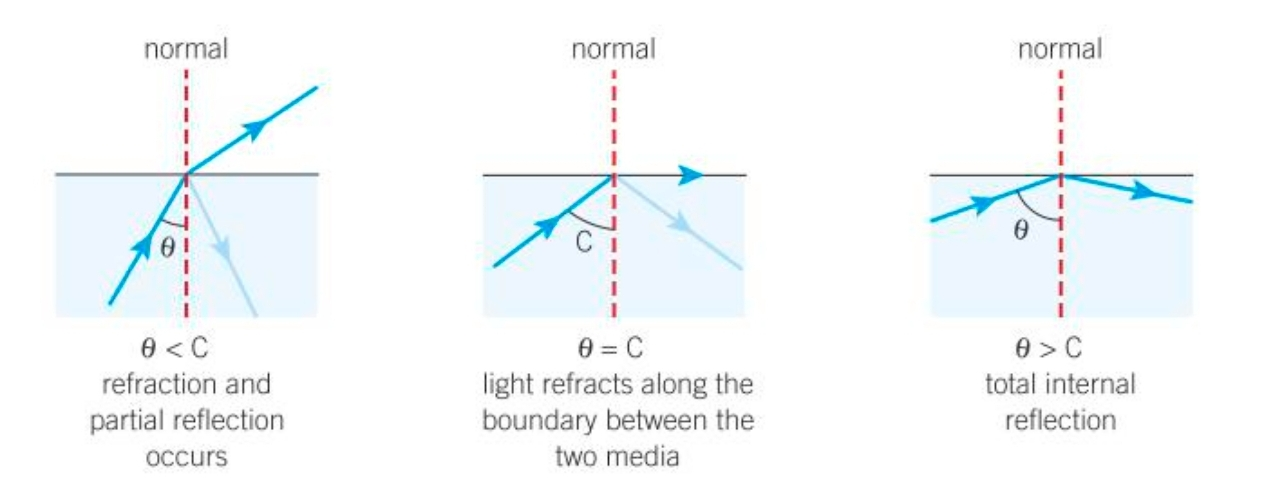
\includegraphics[width=0.8\textwidth]{Waves_Images/criticalangle.jpg}
    \end{figure}
    \begin{itemize}
        \item If $\theta < C$, TIR does not occur, and we use Snell's law as normal
        \item If $\theta = C$, light refracts along the boundary between the two media, and there is a partial reflection
        \item If $\theta > C$, TIR occurs and we use the law of reflection to determine the angle at which it does. 
    \end{itemize}
\end{frame}
\begin{frame}{Examples}
\begin{multicols}{2}
\begin{minipage}{9cm}
    \begin{exampleblock}{Example 1}
    Diamond has a refractive index of 2.42. Calculate the critical angle between the diamond-air boundary. \pause
    --24.4$^\circ$
    \end{exampleblock}
    \end{minipage}
    \columnbreak
    \begin{figure}
\hspace{3cm}
        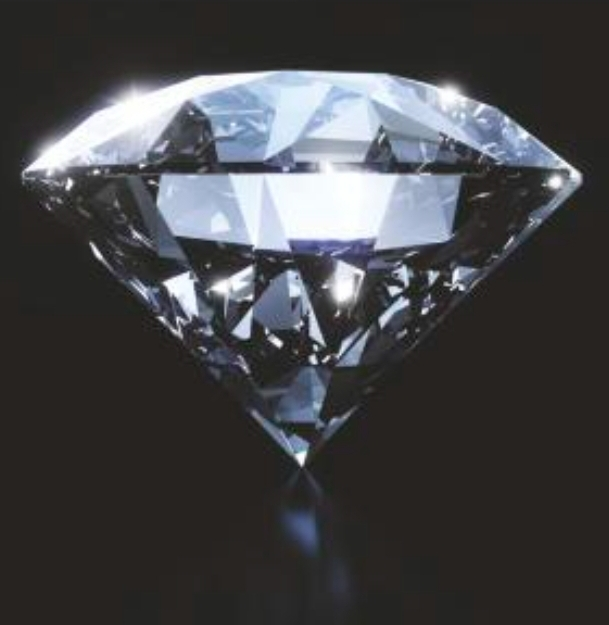
\includegraphics[height=2cm]{Waves_Images/diamond.jpg}
    \end{figure}
    \end{multicols}
    \begin{exampleblock}{Example 2}
    Light travels at a speed of $2.25\times10^8$ ms$^{-1}$ in water. Calculate the refractive index of water, and hence the critical angle at the water-air boundary. \pause
    --$48.8^\circ$
    \end{exampleblock} \pause
    
    \begin{exampleblock}{Example 3}
    A fish tank is made of glass with a refractive index 1.5 and is filled with water (n=1.33). Calculate the critical angle at the water-glass boundary. \pause
    --$62^\circ$
    \end{exampleblock}
\end{frame}

\begin{frame}{Fibre Optics}
    \begin{figure}
        \centering
        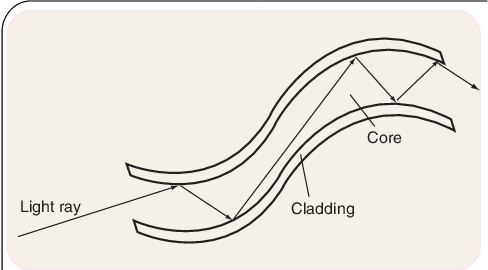
\includegraphics[width=9cm]{Waves_Images/fibreoptics.png}
    \end{figure}
    Fibre Optic cables make use of TIR to transmit digital signals using pulses of light. They have a core with a high refractive index, with a cladding that has a lower RI. This means that the critical angle is low, so very little light can escape, with the cladding providing a second chance to not escape.
\end{frame}

\begin{frame}{Fibre Optics}
    \begin{multicols}{2}

    \begin{itemize}
        \item Uses pulses of light to beam a 0 or 1
        \item More efficient than ordinary copper cables used in communications (no energy losses)
        \item Faster than ordinary cables
        \item Very flexible cables
        \item Can transmit over large distances without loss of signal
        \item Sometimes used for pretty light displays
        
    \end{itemize}
    \columnbreak
    \begin{figure}
        \centering
        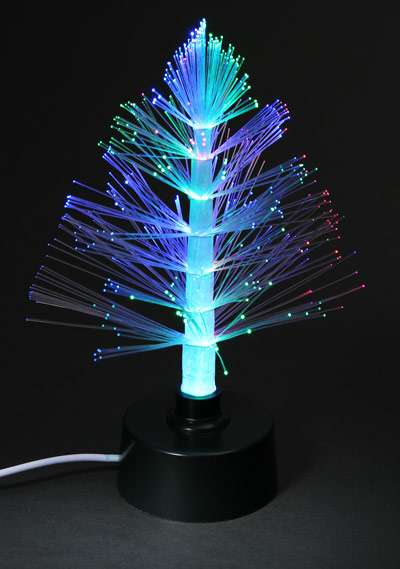
\includegraphics[width=3cm]{Waves_Images/fibreopticchristmastree.png}
    \end{figure}
      \end{multicols}
      \begin{itemize}
      \item But high cost per unit length (compared to copper cables)
        \item Still subject to interference from external light sources - but can be reduced by placing underground
      \end{itemize}
\end{frame}

\end{document}